\documentclass{article}
\usepackage{amsmath}
\usepackage{graphicx}
\usepackage{booktabs}
\usepackage[colorlinks=true, allcolors=blue]{hyperref}
\usepackage[section]{placeins}


\title{Supplementary materials for: Pointing models for users operating under
different speed accuracy strategies }
\author{Anonymous authors}
\date{}
\begin{document}
\maketitle

\section{Intraclass Correlation Coefficients (ICC) for the JGP dataset (Subsection 3.3)}
\subsection{Pearson's $r$}
\begin{center}
    \begin{tabular}{lllrrrrrl}
        \toprule
          & Type  & Description             & ICC      & F        & df1 & df2 & pval     & CI95\%      \\
        \midrule
        0 & ICC1  & Single raters absolute  & 0.278121 & 2.541096 & 14  & 45  & 0.009083 & [0.04 0.59] \\
        1 & ICC2  & Single random raters    & 0.284798 & 2.679707 & 14  & 42  & 0.006876 & [0.05 0.59] \\
        2 & ICC3  & Single fixed raters     & 0.295738 & 2.679707 & 14  & 42  & 0.006876 & [0.05 0.61] \\
        3 & ICC1k & Average raters absolute & 0.606469 & 2.541096 & 14  & 45  & 0.009083 & [0.15 0.85] \\
        4 & ICC2k & Average random raters   & 0.614320 & 2.679707 & 14  & 42  & 0.006876 & [0.18 0.85] \\
        5 & ICC3k & Average fixed raters    & 0.626825 & 2.679707 & 14  & 42  & 0.006876 & [0.18 0.86] \\
        \bottomrule
    \end{tabular}
\end{center}

\subsection{Spearman's $\rho$}
\begin{center}
    \begin{tabular}{lllrrrrrl}
        \toprule
          & Type  & Description             & ICC      & F        & df1 & df2 & pval     & CI95\%      \\
        \midrule
        0 & ICC1  & Single raters absolute  & 0.269582 & 2.476315 & 14  & 45  & 0.010850 & [0.03 0.58] \\
        1 & ICC2  & Single random raters    & 0.272642 & 2.534710 & 14  & 42  & 0.010107 & [0.04 0.58] \\
        2 & ICC3  & Single fixed raters     & 0.277288 & 2.534710 & 14  & 42  & 0.010107 & [0.04 0.59] \\
        3 & ICC1k & Average raters absolute & 0.596174 & 2.476315 & 14  & 45  & 0.010850 & [0.12 0.85] \\
        4 & ICC2k & Average random raters   & 0.599896 & 2.534710 & 14  & 42  & 0.010107 & [0.14 0.85] \\
        5 & ICC3k & Average fixed raters    & 0.605478 & 2.534710 & 14  & 42  & 0.010107 & [0.13 0.85] \\
        \bottomrule
    \end{tabular}

\end{center}


\subsection{Kendall's $\tau$}
\begin{center}
    \begin{tabular}{lllrrrrrl}
        \toprule
          & Type  & Description             & ICC      & F        & df1 & df2 & pval     & CI95\%      \\
        \midrule
        0 & ICC1  & Single raters absolute  & 0.289989 & 2.633714 & 14  & 45  & 0.007048 & [0.05 0.6 ] \\
        1 & ICC2  & Single random raters    & 0.291424 & 2.664110 & 14  & 42  & 0.007166 & [0.05 0.6 ] \\
        2 & ICC3  & Single fixed raters     & 0.293799 & 2.664110 & 14  & 42  & 0.007166 & [0.05 0.6 ] \\
        3 & ICC1k & Average raters absolute & 0.620308 & 2.633714 & 14  & 45  & 0.007048 & [0.18 0.86] \\
        4 & ICC2k & Average random raters   & 0.621946 & 2.664110 & 14  & 42  & 0.007166 & [0.18 0.86] \\
        5 & ICC3k & Average fixed raters    & 0.624640 & 2.664110 & 14  & 42  & 0.007166 & [0.18 0.86] \\
        \bottomrule
    \end{tabular}
\end{center}

\section{Association measures for the GO dataset (Subsection 4.3)}

\begin{figure}[htbp]
    \centering
    \includegraphics[width=.8\textwidth]{img/association_gop_agg_strategy.pdf}
    \caption{<caption>}
    \label{<label>}
\end{figure}
\begin{table}
    \centering
    \caption{}
    \begin{tabular}{lrrr}
        \toprule
                 & r        & rho      & tau      \\
        strategy &          &          &          \\
        \midrule
        1        & 0.027881 & 0.034877 & 0.019789 \\
        2        & 0.111236 & 0.116360 & 0.085362 \\
        3        & 0.266716 & 0.262616 & 0.193317 \\
        4        & 0.093823 & 0.107219 & 0.077531 \\
        5        & 0.217365 & 0.226004 & 0.173897 \\
        \bottomrule
    \end{tabular}
\end{table}


\section{Linear fits for the Gaussian bivariate fit per strategy for the GO dataset (Subsection 4.5)}
\subsection{$\mu_i = \text{const} + x_1\,\text{strategy}$}
\begin{center}
    \begin{tabular}{lclc}
        \toprule
        \textbf{Dep. Variable:}    & y                & \textbf{  R-squared:         } & 0.934   \\
        \textbf{Model:}            & OLS              & \textbf{  Adj. R-squared:    } & 0.912   \\
        \textbf{Method:}           & Least Squares    & \textbf{  F-statistic:       } & 42.58   \\
        \textbf{Date:}             & Tue, 10 Sep 2024 & \textbf{  Prob (F-statistic):} & 0.00731 \\
        \textbf{Time:}             & 16:31:51         & \textbf{  Log-Likelihood:    } & 3.4797  \\
        \textbf{No. Observations:} & 5                & \textbf{  AIC:               } & -2.959  \\
        \textbf{Df Residuals:}     & 3                & \textbf{  BIC:               } & -3.741  \\
        \textbf{Df Model:}         & 1                & \textbf{                     } &         \\
        \textbf{Covariance Type:}  & nonrobust        & \textbf{                     } &         \\
        \bottomrule
    \end{tabular}
    \begin{tabular}{lcccccc}
                       & \textbf{coef} & \textbf{std err} & \textbf{t} & \textbf{P$> |$t$|$} & \textbf{[0.025} & \textbf{0.975]} \\
        \midrule
        \textbf{const} & 1.2957        & 0.070            & 18.602     & 0.000               & 1.074           & 1.517           \\
        \textbf{x1}    & 0.6428        & 0.099            & 6.525      & 0.007               & 0.329           & 0.956           \\
        \bottomrule
    \end{tabular}
    \begin{tabular}{lclc}
        \textbf{Omnibus:}       & nan   & \textbf{  Durbin-Watson:     } & 1.778 \\
        \textbf{Prob(Omnibus):} & nan   & \textbf{  Jarque-Bera (JB):  } & 0.441 \\
        \textbf{Skew:}          & 0.048 & \textbf{  Prob(JB):          } & 0.802 \\
        \textbf{Kurtosis:}      & 1.548 & \textbf{  Cond. No.          } & 1.41  \\
        \bottomrule
    \end{tabular}
    %\caption{OLS Regression Results}
\end{center}

Notes: \newline
[1] Standard Errors assume that the covariance matrix of the errors is correctly specified.



\subsection{$\mu_t = \text{const} + x_1\,\text{strategy}$}
\begin{center}
    \begin{tabular}{lclc}
        \toprule
        \textbf{Dep. Variable:}    & y                & \textbf{  R-squared:         } & 0.934   \\
        \textbf{Model:}            & OLS              & \textbf{  Adj. R-squared:    } & 0.912   \\
        \textbf{Method:}           & Least Squares    & \textbf{  F-statistic:       } & 42.58   \\
        \textbf{Date:}             & Tue, 10 Sep 2024 & \textbf{  Prob (F-statistic):} & 0.00731 \\
        \textbf{Time:}             & 16:31:51         & \textbf{  Log-Likelihood:    } & 3.4797  \\
        \textbf{No. Observations:} & 5                & \textbf{  AIC:               } & -2.959  \\
        \textbf{Df Residuals:}     & 3                & \textbf{  BIC:               } & -3.741  \\
        \textbf{Df Model:}         & 1                & \textbf{                     } &         \\
        \textbf{Covariance Type:}  & nonrobust        & \textbf{                     } &         \\
        \bottomrule
    \end{tabular}
    \begin{tabular}{lcccccc}
                       & \textbf{coef} & \textbf{std err} & \textbf{t} & \textbf{P$> |$t$|$} & \textbf{[0.025} & \textbf{0.975]} \\
        \midrule
        \textbf{const} & 1.2957        & 0.070            & 18.602     & 0.000               & 1.074           & 1.517           \\
        \textbf{x1}    & 0.6428        & 0.099            & 6.525      & 0.007               & 0.329           & 0.956           \\
        \bottomrule
    \end{tabular}
    \begin{tabular}{lclc}
        \textbf{Omnibus:}       & nan   & \textbf{  Durbin-Watson:     } & 1.778 \\
        \textbf{Prob(Omnibus):} & nan   & \textbf{  Jarque-Bera (JB):  } & 0.441 \\
        \textbf{Skew:}          & 0.048 & \textbf{  Prob(JB):          } & 0.802 \\
        \textbf{Kurtosis:}      & 1.548 & \textbf{  Cond. No.          } & 1.41  \\
        \bottomrule
    \end{tabular}
    %\caption{OLS Regression Results}
\end{center}

Notes: \newline
[1] Standard Errors assume that the covariance matrix of the errors is correctly specified.


\subsection{$\sigma_i = \text{const} + x_1\,\text{strategy}$}

\begin{center}
    \begin{tabular}{lclc}
        \toprule
        \textbf{Dep. Variable:}    & y                & \textbf{  R-squared:         } & 0.590   \\
        \textbf{Model:}            & OLS              & \textbf{  Adj. R-squared:    } & 0.453   \\
        \textbf{Method:}           & Least Squares    & \textbf{  F-statistic:       } & 4.317   \\
        \textbf{Date:}             & Tue, 10 Sep 2024 & \textbf{  Prob (F-statistic):} & 0.129   \\
        \textbf{Time:}             & 16:31:51         & \textbf{  Log-Likelihood:    } & 1.6774  \\
        \textbf{No. Observations:} & 5                & \textbf{  AIC:               } & 0.6452  \\
        \textbf{Df Residuals:}     & 3                & \textbf{  BIC:               } & -0.1360 \\
        \textbf{Df Model:}         & 1                & \textbf{                     } &         \\
        \textbf{Covariance Type:}  & nonrobust        & \textbf{                     } &         \\
        \bottomrule
    \end{tabular}
    \begin{tabular}{lcccccc}
                       & \textbf{coef} & \textbf{std err} & \textbf{t} & \textbf{P$> |$t$|$} & \textbf{[0.025} & \textbf{0.975]} \\
        \midrule
        \textbf{const} & 1.0564        & 0.100            & 10.576     & 0.002               & 0.739           & 1.374           \\
        \textbf{x1}    & 0.2935        & 0.141            & 2.078      & 0.129               & -0.156          & 0.743           \\
        \bottomrule
    \end{tabular}
    \begin{tabular}{lclc}
        \textbf{Omnibus:}       & nan    & \textbf{  Durbin-Watson:     } & 1.799 \\
        \textbf{Prob(Omnibus):} & nan    & \textbf{  Jarque-Bera (JB):  } & 0.816 \\
        \textbf{Skew:}          & -0.387 & \textbf{  Prob(JB):          } & 0.665 \\
        \textbf{Kurtosis:}      & 1.178  & \textbf{  Cond. No.          } & 1.41  \\
        \bottomrule
    \end{tabular}
    %\caption{OLS Regression Results}
\end{center}

Notes: \newline
[1] Standard Errors assume that the covariance matrix of the errors is correctly specified.

\subsection{$\sigma_t = \text{const} + x_1\,\text{strategy}$}

\begin{center}
    \begin{tabular}{lclc}
        \toprule
        \textbf{Dep. Variable:}    & y                & \textbf{  R-squared:         } & 0.681  \\
        \textbf{Model:}            & OLS              & \textbf{  Adj. R-squared:    } & 0.574  \\
        \textbf{Method:}           & Least Squares    & \textbf{  F-statistic:       } & 6.396  \\
        \textbf{Date:}             & Tue, 10 Sep 2024 & \textbf{  Prob (F-statistic):} & 0.0855 \\
        \textbf{Time:}             & 16:31:52         & \textbf{  Log-Likelihood:    } & 9.2180 \\
        \textbf{No. Observations:} & 5                & \textbf{  AIC:               } & -14.44 \\
        \textbf{Df Residuals:}     & 3                & \textbf{  BIC:               } & -15.22 \\
        \textbf{Df Model:}         & 1                & \textbf{                     } &        \\
        \textbf{Covariance Type:}  & nonrobust        & \textbf{                     } &        \\
        \bottomrule
    \end{tabular}
    \begin{tabular}{lcccccc}
                       & \textbf{coef} & \textbf{std err} & \textbf{t} & \textbf{P$> |$t$|$} & \textbf{[0.025} & \textbf{0.975]} \\
        \midrule
        \textbf{const} & 0.3852        & 0.022            & 17.424     & 0.000               & 0.315           & 0.456           \\
        \textbf{x1}    & 0.0791        & 0.031            & 2.529      & 0.085               & -0.020          & 0.179           \\
        \bottomrule
    \end{tabular}
    \begin{tabular}{lclc}
        \textbf{Omnibus:}       & nan   & \textbf{  Durbin-Watson:     } & 1.787 \\
        \textbf{Prob(Omnibus):} & nan   & \textbf{  Jarque-Bera (JB):  } & 0.759 \\
        \textbf{Skew:}          & 0.358 & \textbf{  Prob(JB):          } & 0.684 \\
        \textbf{Kurtosis:}      & 1.231 & \textbf{  Cond. No.          } & 1.41  \\
        \bottomrule
    \end{tabular}
    %\caption{OLS Regression Results}
\end{center}

Notes: \newline
[1] Standard Errors assume that the covariance matrix of the errors is correctly specified.

\subsection{$\rho = \text{const} + x_1\,\text{strategy}$}

\begin{center}
    \begin{tabular}{lclc}
        \toprule
        \textbf{Dep. Variable:}    & y                & \textbf{  R-squared:         } & 0.565  \\
        \textbf{Model:}            & OLS              & \textbf{  Adj. R-squared:    } & 0.420  \\
        \textbf{Method:}           & Least Squares    & \textbf{  F-statistic:       } & 3.896  \\
        \textbf{Date:}             & Tue, 10 Sep 2024 & \textbf{  Prob (F-statistic):} & 0.143  \\
        \textbf{Time:}             & 16:31:52         & \textbf{  Log-Likelihood:    } & 3.0488 \\
        \textbf{No. Observations:} & 5                & \textbf{  AIC:               } & -2.098 \\
        \textbf{Df Residuals:}     & 3                & \textbf{  BIC:               } & -2.879 \\
        \textbf{Df Model:}         & 1                & \textbf{                     } &        \\
        \textbf{Covariance Type:}  & nonrobust        & \textbf{                     } &        \\
        \bottomrule
    \end{tabular}
    \begin{tabular}{lcccccc}
                       & \textbf{coef} & \textbf{std err} & \textbf{t} & \textbf{P$> |$t$|$} & \textbf{[0.025} & \textbf{0.975]} \\
        \midrule
        \textbf{const} & 0.3447        & 0.076            & 4.539      & 0.020               & 0.103           & 0.586           \\
        \textbf{x1}    & 0.2119        & 0.107            & 1.974      & 0.143               & -0.130          & 0.554           \\
        \bottomrule
    \end{tabular}
    \begin{tabular}{lclc}
        \textbf{Omnibus:}       & nan   & \textbf{  Durbin-Watson:     } & 1.648 \\
        \textbf{Prob(Omnibus):} & nan   & \textbf{  Jarque-Bera (JB):  } & 0.479 \\
        \textbf{Skew:}          & 0.485 & \textbf{  Prob(JB):          } & 0.787 \\
        \textbf{Kurtosis:}      & 1.833 & \textbf{  Cond. No.          } & 1.41  \\
        \bottomrule
    \end{tabular}
    %\caption{OLS Regression Results}
\end{center}

Notes: \newline
[1] Standard Errors assume that the covariance matrix of the errors is correctly specified.


\section{Values of the t-copula for the GO dataset, effect of strategy and participants}

\begin{figure}[htbp]
    \centering
    \makebox[\textwidth]{
        \includegraphics[width=1.3\textwidth]{img/tcop_values.pdf}
    }
    \caption{<caption>}
    \label{<label>}
\end{figure}

\begin{table}
    \caption{Mixed Linear Model Regression Results}
    \label{}
    \begin{center}
        \begin{tabular}{llll}
            \hline
            Model:            & MixedLM & Dependent Variable: & rho1    \\
            No. Observations: & 72      & Method:             & REML    \\
            No. Groups:       & 15      & Scale:              & 0.0119  \\
            Min. group size:  & 4       & Log-Likelihood:     & 46.7778 \\
            Max. group size:  & 5       & Converged:          & Yes     \\
            Mean group size:  & 4.8     &                     &         \\
            \hline
        \end{tabular}
    \end{center}

    \begin{center}
        \begin{tabular}{lrrrrrr}
            \hline
                      & Coef.  & Std.Err. & z      & P$> |$z$|$ & [0.025 & 0.975] \\
            \hline
            Intercept & 0.773  & 0.026    & 30.251 & 0.000      & 0.723  & 0.823  \\
            strategy  & -0.012 & 0.009    & -1.312 & 0.189      & -0.030 & 0.006  \\
            Group Var & 0.002  & 0.018    &        &            &        &        \\
            \hline
        \end{tabular}
    \end{center}
\end{table}




\section{Correction on $\beta_0$ instead of $\lambda_1$ for Model 3 (Subsection 6.1)}

\begin{figure}[htbp]
    \centering
    \makebox[\textwidth]{
        \includegraphics[width=1.3\textwidth]{img/method_consistency_correct_beta.pdf}
    }
    \caption{<caption>}
    \label{<label>}
\end{figure}

\section{Replications of Figure 7 with different seeds (Subsection 6.1)}

\begin{figure}[htbp]
    \centering
    \makebox[\textwidth]{
        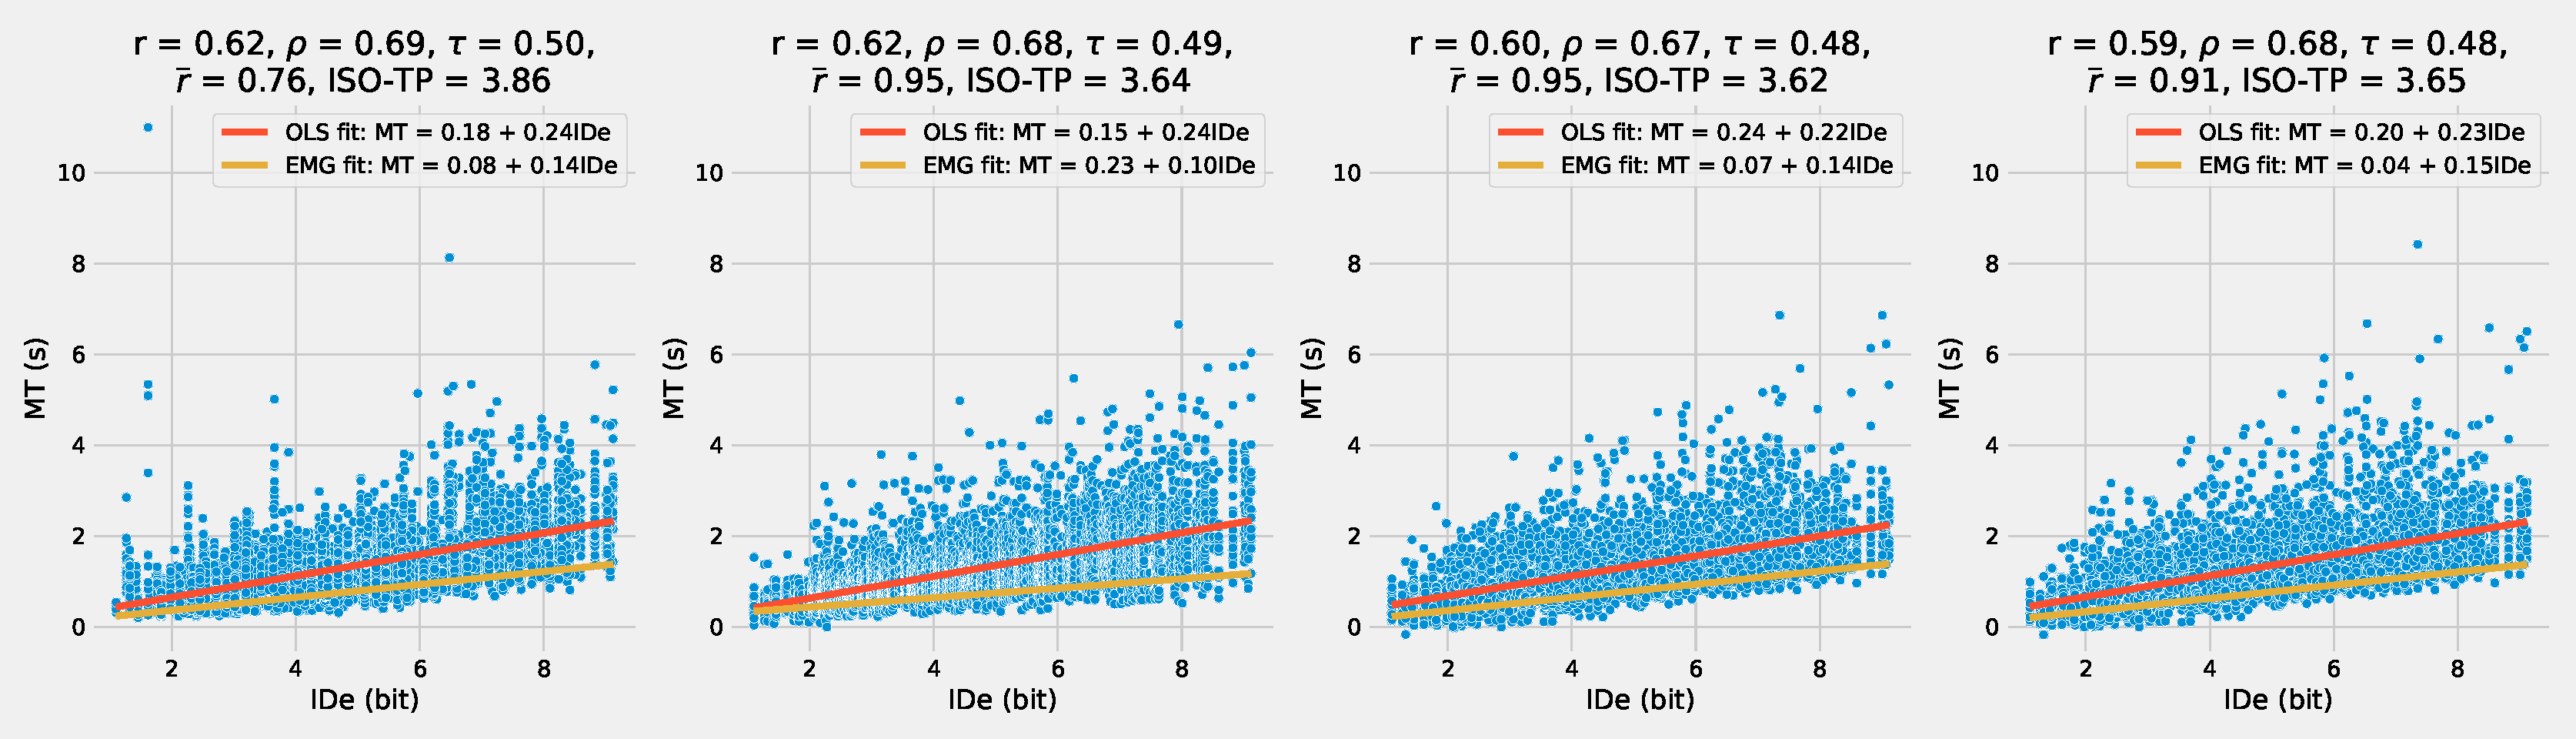
\includegraphics[width=1.3\textwidth]{img/method_consistency_seed777.pdf}
    }
    \caption{Seed = 777}
    \label{<label>}
\end{figure}
\begin{figure}[htbp]
    \centering
    \makebox[\textwidth]{
        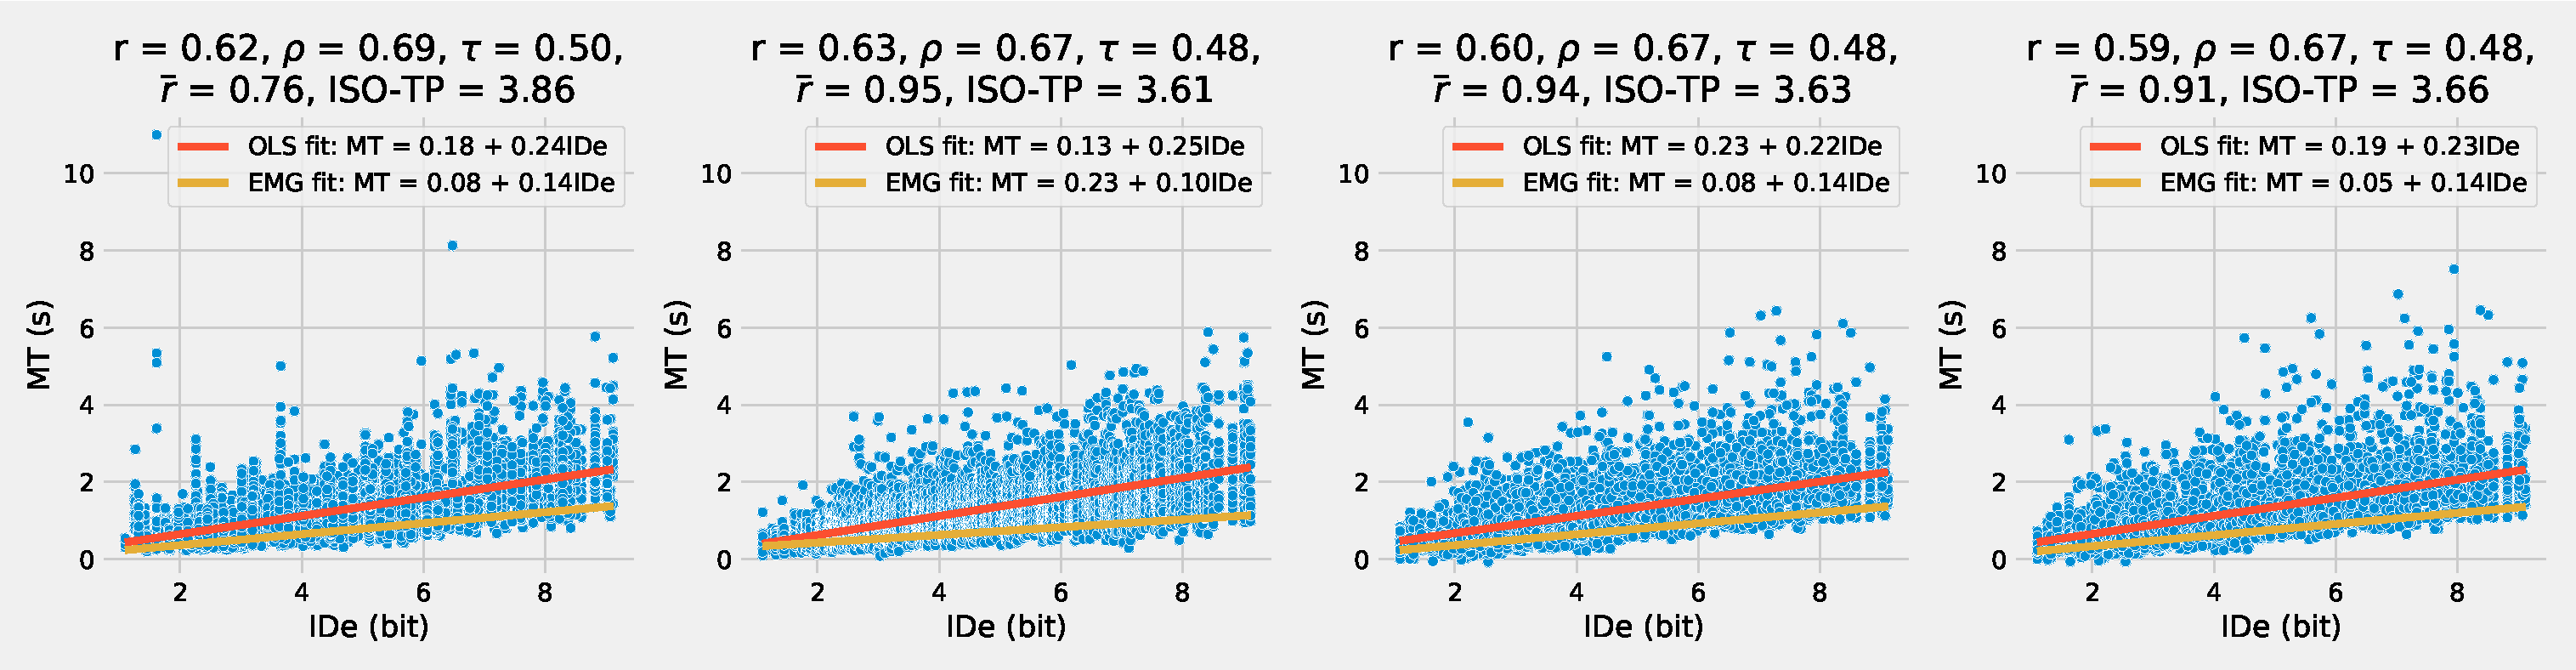
\includegraphics[width=1.3\textwidth]{img/method_consistency_seed999.pdf}
    }
    \caption{Seed = 999}
    \label{<label>}
\end{figure}
\begin{figure}[htbp]
    \centering
    \makebox[\textwidth]{
        \includegraphics[width=1.3\textwidth]{img/method_consistency_seedNone.pdf}
    }
    \caption{Seed = None}
    \label{<label>}
\end{figure}

\section{Participant internal consistency concerning strategies}

\begin{figure}[htbp]
    \centering
    \includegraphics[width=.48\textwidth]{img/fitts_gop_1.pdf}
    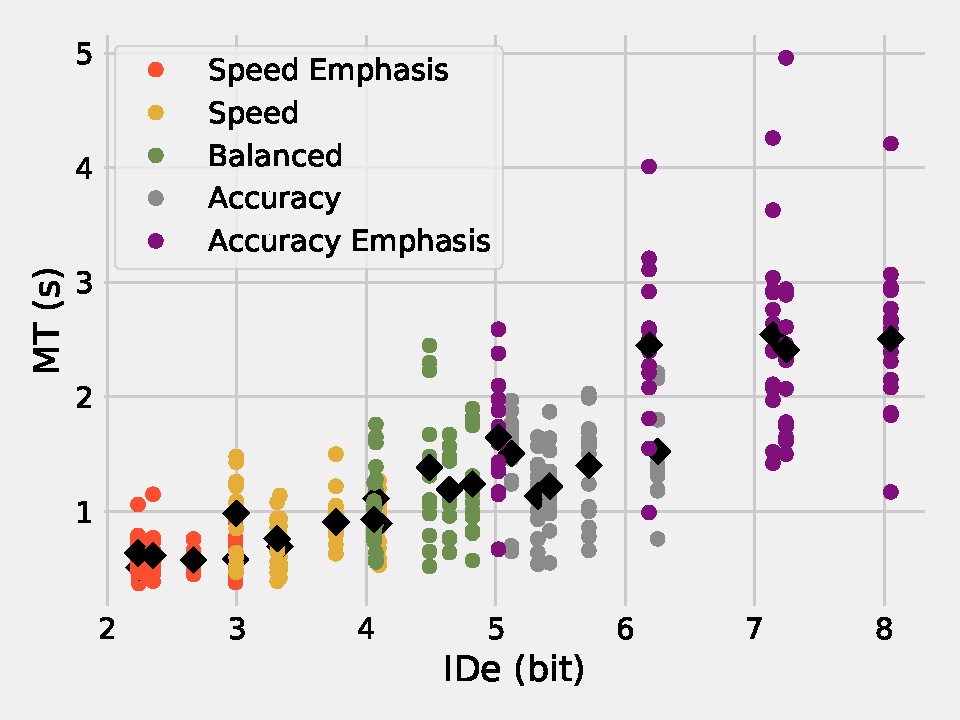
\includegraphics[width=.48\textwidth]{img/fitts_gop_2.pdf} \\
    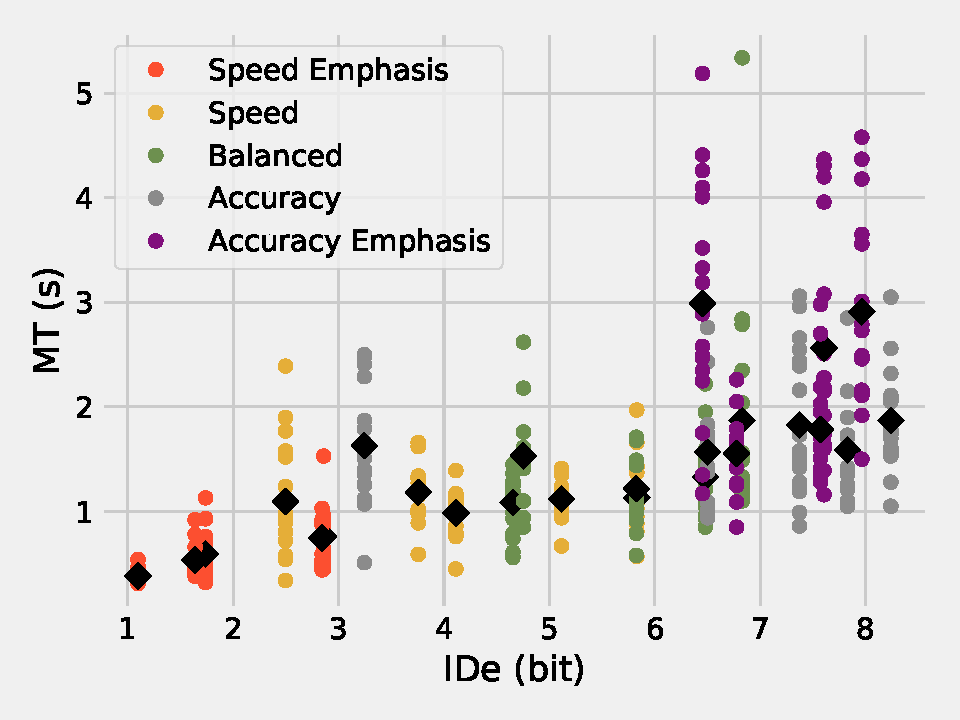
\includegraphics[width=.48\textwidth]{img/fitts_gop_10.pdf}
    \includegraphics[width=.48\textwidth]{img/fitts_gop_16.pdf}
    \caption{<caption>}
    \label{<label>}
\end{figure}


\end{document}